% !TEX program = xelatex


\documentclass{article} 
\usepackage{xltxtra} % 这个包是为了打印\XeLaTeX 的Logo。 
\usepackage{xeCJK} % 这个包可以指定中文字体。
\setCJKmainfont[Mapping=tex-text,BoldFont=SimHei]{SimSun}
\setCJKsansfont{SimHei}
\setCJKmonofont[Scale=.85]{FandolFang}
\setmainfont{Palatino Linotype}
\setmonofont{Consolas}

\usepackage{url}
\usepackage{geometry}
\geometry{left=3cm,right=3cm}

\newcommand{\e}[1]{$ \times 10^{#1}$}
\renewcommand{\figurename}{图}
\renewcommand{\tablename}{表}
\renewcommand{\today}{\number\year 年 \number\month 月 \number\day 日}



\begin{document}
 \title{Recommder System Handbook学习笔记\ 第一部分,章节2 推荐系统中的数据挖掘方法}
 \author{littlekideee}
 \maketitle
 \section{介绍}
 推荐系统核心算法来自数据挖掘技术。

 典型的数据挖掘包含三步:数据处理,数据分析和结果解释。
 \begin{figure}[htb]
	  \begin{center}
	  	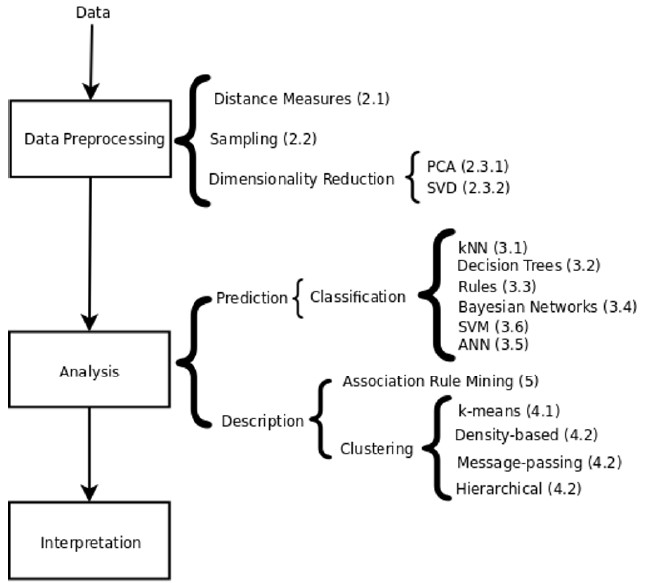
\includegraphics[scale=0.6]{f2.1.jpg}
	  	\caption{数据挖掘问题中的主要步骤和方法。}
	  \end{center}
 \end{figure}

 \section{数据预处理}
 我们把数据定义为对象和它们属性的集合。

 本节主要关注当设计一个推荐系统的时候的三个重要问题。首先,复习一下相似度或距离计算方法,然后,讨论纵大量数据中采样的问题,最后,讨论降维的通用技术。

 \subsection{相似度度量方法}
 1.欧式距离
 $$ d(x,y)=\sqrt{\mathop{\sum}_{k=1}^n(x_k-y_k)^2} $$

 其中,$ n $是维(属性)数,$ x_k $和$ y_k $是数据对象想x和y的第$ k $个属性。

 2.Minkowski距离
 $$ d(x,y)=({\mathop{\sum}_{k=1}^n|x_k-y_k|^r)^\frac{1}{r}} $$

 其中r是距离的度。r值得不同,Minkowski距离有不同的名字:$r=1$:city block(曼哈顿距离),$r=2$:欧氏距离,$r\rightarrow\infty$:supremum距离,这个距离计算数据对象的某些维度之间最大不同。

 3.Mahalanobis距离
 $$ d(x,y)=\sqrt{(x-y)\sigma^{-1}(x-y)^T} $$

 这里,$\sigma$是数据的协方差矩阵。

 4.余弦相似度
 $$ cos(x,y)=\frac{x\bullet y}{\|x\|\|y\|} $$

 5.皮尔逊相关系数
 $$ Pearson(x,y)=\frac{\sum(x,y)}{\sigma_x\times\sigma_y} $$

 RS中使用的是余弦相似度和皮尔逊相似度,Spertus等人做实验发现余弦相似度效果最好。Lathia等人实验结果显示RS的预测准确度与相似度方法的选择关系不大。

 另外,当项目仅包含2元属性时,有几个特殊的相似度度量方法。首选计算四个值:$M01$,$M10$,$M11$,$M00$=x为0,y为1的属性数量,以此类推。我们可以计算1.简单搭配系数 $ SMC=\frac{number\ of\ matches}{number\ of\ attributes}=\frac{M11+M00}{M01+M10+M11+M00} $;2.Jaccard系数$JC=\frac{M11}{M01+M10+M11}$。以及Jaccard的一种变化(Tanimoto):$ d=\frac{x\bullet y}{\|x\|^2+\|x\|^2-x\bullet y} $。

 \subsection{采样}
 采样(Sampling)是DM中从大数据集中选择相关数据子集的一种主要技术。Sampling还可以用来创建训练集和测试集。训练集用来学习参数和算法的配置。测试集用来评估模型和训练阶段得到的配置数据来确保未观测到的数据在模型上也表现得很好。

 采样的关键问题是得到的子集是否具有代表性。最简单的采样技术就是随机采样,等概率的抽取数据。此外,还有其他的随机方法。比如,在分层(stratified)采样中,吧数据根据特定的特征划分成几个部分,然后在几个部分上独立随机采样。

 现在比较通用的方法是使用标准不放回随机抽样,80/20划分训练集和测试集。

 为避免划分数据集的采样导致过度专一化(over-specialization),训练过程应该重复几次。不同的训练集/测试集用来重复训练/测试K次。最终,取K次试验的平均成果。这个过程就是交叉验证机制。有几个交叉验证技术:1.重复随机采样,把标准随机采样重复K次。2.n-fold交叉验证,数据集被分成n个folds,一个fold用来测试模型,其余n-1个用来训练模型。然后交叉验证过程被重复n次,每次使用不同的子样本作为验证集。3.leave-one-out(LOO)方法,它可以被视为n-Fold的极端情况,它把每个样本单独做为验证集。

 \subsection{降维}
 稀疏性和维数灾难问题常常出现在RS中。因此,降维技术非常有必要。

 RS中最常用的两个降维技术:1.主成分分析(PCA),2.奇异值分解(SVD)。

 \subsubsection{PCA}
 PCA是一种经典的发现高维数据中的模式的统计方法。

 第一成分的方差的量是大于第二成分方差的量的。我们可以通过忽略掉那些在方差上贡献较小的成分来达到降维的目的。

 图2显示了二维高斯联合分布点云的PCA分析。在数据聚集之后,主成分被计算为$u_1$和$u_2$。注意新坐标的长度是他们特征向量中包含的能量。由图2的例子,第一个成分$u_1$包含了83.5\%的能量,这意味着移除成分$u_2$仅仅损失16.5\%的信息。一般而言,选择$m^{'}$个成分,使之能量累积超过特定的阈值,一般为90\%。
 \begin{figure}[!htb]
	  \begin{center}
	  	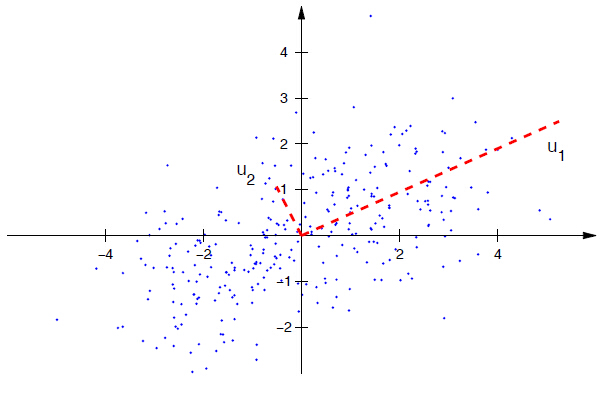
\includegraphics[scale=0.6]{f2.2.jpg}
	  	\caption{二维高斯联合分布点云的PCA分析。}
	  \end{center}
 \end{figure}


 \subsubsection{SVD}
 奇异值分解是一种强力的降维技术。SVD降维的关键问题是找到一个低维特征空间,它能代表一些语义概念信息。(在LSA中是一种基础方法)

 SVD算法的核心依赖于如下理论:

 给出一个矩阵$A$,总能分解成$A=U\lambda V^T$。给一个$n\times m$的矩阵$A$(n个项目,m个特征),我们能获得一个$n\times r$的矩阵$U$(n个项目,r个概念),和一个$r\times r$的对角阵$\lambda$(概念的强度),以及一个$m\times r$的矩阵$V$(m个特征,r个概念)。

 \begin{figure}[htb]
	  \begin{center}
	  	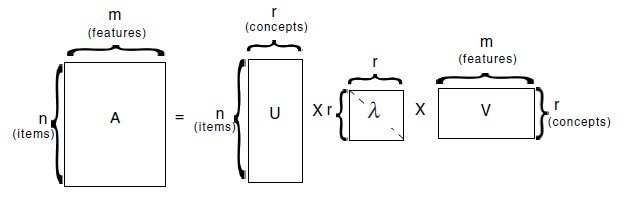
\includegraphics[scale=0.6]{f2.3.jpg}
	  	\caption{Illustrating the basic Singular Value Decomposition Theorem: an item $\times$ features matrix can be decomposed into three different ones: an item $\times$ concepts, aconcept strength, and a concept $\times$ features.}
	  \end{center}
 \end{figure}
把r个特征值降序排列,取前k个,这样就得到了rank-k的A矩阵的近似矩阵$A_k=U_k\lambda_kV_k^T$。
 
SVD有两个使用方式,第一种是利用SVD寻找用户-产品之间的潜在关系,从而预测评分。第二种是利用SVD的产生的低维空间提高近邻方法的精度。

SVD的优点是当新加入的数据时,不需要重新计算模型。SVD方法在Netflix大赛中取得了巨大的成功。

顺带一提,还有很多MF的方法,如非负矩阵分解(NNMF)等。这些方法和SVD十分相似。

\subsection{去噪}
原始数据中可能有一些不同的噪声,比如丢失的值或无用的数据等。因此,降噪是去除数据中不良影响,最大化数据信息量的重要过程。

在RS中,主要区分两类噪声:natural和malicious(恶意的)。

malicious噪声能够影响RS的输出。而natural噪声对RS的表现的影响可以忽略不计。

\section{分类}
一个分类器是将特征空间映射到标签空间中,举一个餐馆的例子,根据描述餐馆的一系列特征,它们可以被分为(good,bad)两类。

有两种分类:1.有监督的,即标签或类目是已知的。2.无监督的,即标签或类目是未知的。

\subsection{最近邻}
第一种是基于实例的分类器,通常也叫做最近邻分类器(kNN)。如果要给一个点分类,kNN分类器从训练数据中寻找它的k个最近的点,然后依赖最近的这些点给予标记。

给出一个需要分类的点$q$,和一个训练集$ X=\{\{x_1,l_1\}\dots\{x_n\}\} $,$x_j$是第j个元素,$l_j$是它的标签,然后寻找到一个k最近邻的子集$ Y=\{\{y_1,l_1\}\dots\{y_n\}\} $,其中$Y\in X$而且$\sum_1^kd(q,y_k)$是最小的。Y中包含了X中与$q$最接近的k个点。然后,$q$可以标记为$l=f(\{l_1\dots l_k\})$。
\begin{figure}[!htb]
	  \begin{center}
	  	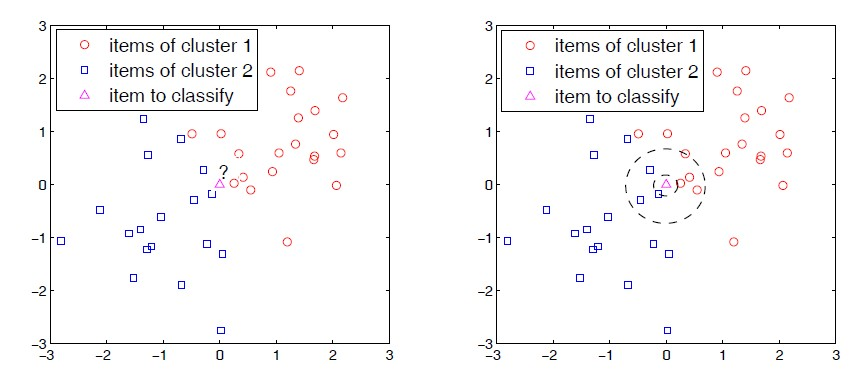
\includegraphics[scale=0.5]{f2.4.jpg}
	  	\caption{k近邻的例子。}
	  \end{center}
\end{figure}

可能现在kNN最大的挑战就是$k$的选择。如果$k$太小,那么分类器就会对噪声点十分敏感,反之,如果$k$太大,邻域内就会包含太多其他类的点。

kNN在RS中被广泛使用,在CF中,寻找相似的用户或项目。而且它还具有惰性学习的优点,维护模型的成本低。

\subsection{决策树}
决策树是以树结构组织目标属性或类的分类器。决策树包含两类节点a)决策节点,决定目标属性属于那一颗子树,b)叶子节点,显示目标属性的值

通常的一些决策树:Hunts Algorithm,CART,ID3,C4.5,SLIQ,SPRINT。其中Hunt Algorithm是最早也是最容易理解的。

决策树的划分策略可以根据最大化信息增益得到:
$$ \Delta_i=I(parent)-\mathop{\sum}\limits_{j=1}^{k_i}\frac{N(v_j)I(v_j)}{N} $$

其中,$k_i$是属性$i$的值,$N$是观察的到的数量,$v_j$是根据属性$i$值的第$j$个划分。除此之外,还有一种度量方法是Gini指数。

决策树迭停止条件是所有观测值都属于同一类。但在实践中,我们需要对庞大的决策树进行剪枝操作,简化决策树的复杂度。

使用决策树构建分类器的主要优点是消耗低,对未知实例分类的速度快。

决策树可能会用于基于模型的RS方法中。一种可能性是使用内容特征去建立一个决策树,它将所有与用户偏好有关的变量都建模。另外,决策树还可以作为RS的一部分,比如它可以过滤一部分用户。

\subsection{基于规则的分类器}
基于规则的分类器使用“if...then...”规则的集合来分类数据。规则的前提或是条件是属性连词的表达式。规则的结论是一个正或者负的分类。

如果对象的属性满足规则的条件,我们可以说规则R覆盖对象x。我们定义规则的覆盖性为满足前提的部分记录。另一方面,我们定义准确性为既满足前提又满足结论的部分记录。如果规则彼此之间是独立的,我们说分类器包含互斥的规则(mutually exclusive rules)。最后,如果属性值得所有可能组合都被覆盖的话,即,一个记录至少被一个规则覆盖,我们认为分类器具有详尽规则(exhausitive rules)。

为了建立一个基于规则的分类器,我们可以用从数据中直接抽取规则的直接方法。这种方法的例子是RIPPER,或CN2。另一方面,使用间接的方法从其它分类模型中抽取规则很常见,例如:决策树模型或是神经模型。

基于规则分类器的优点是它们表示很明确,因为它们是符号化的并且可以在没有任何转化的情况下操作数据的属性。

但是,与决策树方法类似,建立一个完整基于规则的推荐模型是很难的。事实上,这种方法在推荐的环境中不是很流行,因为得到一个基于规则的系统意味着我们要么具有一些决策过程中的显式的先验知识,要么我们从另一个模型中提取规则,例如决策树。但是基于规则的系统通过注入一些领域知识或者是商业规则来提高推荐系统的性能。

\subsection{贝叶斯分类器}
贝叶斯分类器是解决分类问题的一个概率框架。它基于条件概率和贝叶斯理论。贝叶斯学派使用概率来代表从数据中学习到的关系的不确定性。先验代表了我们的期望值,或者真正关系可能是什么的先验知识。特别地,给定数据后,模型的概率(后验概率)是与似然值乘以先验概率的乘积成比例的。似然值部分包含了数据的影响,而先验概率则表明观测数据之前模型的可信度。

贝叶斯分类器把每个属性和类标签都看做随机变量。给定一个具有$N$个属性($A_1,A_2,\dots,A_N$)的记录,目标预测类$C_k$,方法是在给定数据$P(C_k|A_1,A_2,\dots,A_N)$,找到能够最大化该类后验概率的$C_k$的值。应用贝叶斯理论,$P(C_k|A_1,A_2,\dots,A_N)\propto P(A_1,A_2,\dots,A_N|C_k)P(C_k)$。

一个特殊但是最常用的分类器是朴素贝叶斯分类器。它假设属性的概率是相互独立的:$P(A_1,A_2,\dots,A_N|C_k)=P(A_1|C_k)P(A_2|C_k)\dots P(A_N|C_k)$。

朴素贝叶斯的主要好处是,受孤立噪音点和不相关的属性的影响小,并且在概率估算期间可以通过忽略实例来处理缺失值。但是,独立性假设对一些相互关联的属性来说可能不成立。在这种情况下,通常的方法是使用所谓的贝叶斯信念网络(BBN)(或是简称贝叶斯网络)。BBN使用非循环图表示属性之间的依赖性,并使用概率表表示结点与直接父亲之间的联系。和朴素贝叶斯分类器方法类似,BBN可以很好地处理不完整的数据,对于模型的过拟合有相当的健壮性。

贝叶斯分类器在基于模型的推荐系统中特别受欢迎。它们经常被用来为基于内容的推荐生成模型。当然,它们也被用于协同环境中。

\subsection{人工神经网络}
人工神经网络(ANN)由一组内连接点和带权链接组成,其想法来自于生物大脑的结构。ANN中的节点被称为神经元,类似于生物神经。这些简单的功能单元组成网络,网络在用有效数据训练之后能够学习分类问题。
\begin{figure}[!htb]
	  \begin{center}
	  	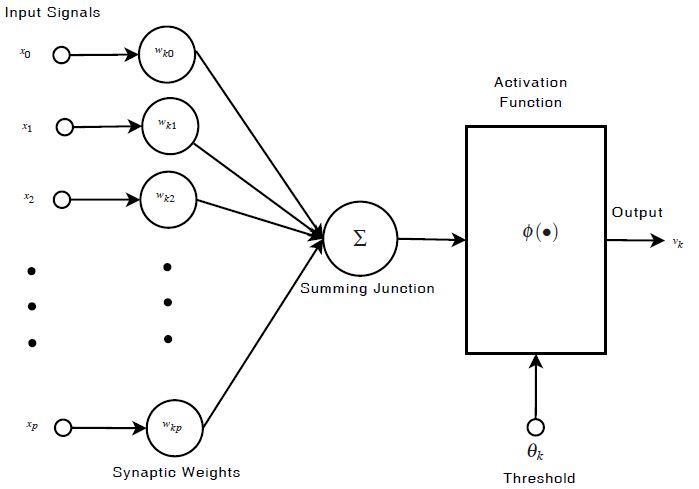
\includegraphics[scale=0.5]{f2.5.jpg}
	  	\caption{感知器模型}
	  \end{center}
\end{figure}

ANN的最简单模型是感知器模型,如图5所示。如果我们把激活函数$\phi$特指为简单的阈值函数,则输出就是根据每条链接的权重将输入值累加,然后和某个阈值$\theta_K$相比较。输出函数为:
\[
y_k=\left\{
\begin{array}{ll}
1,\  & if \sum x_iw_{ki}\geq\theta_k \\
0,\  & if \sum x_iw_{ki}<\theta_k
\end{array}
\right.
\]

感知模型是具有简单和有效学习算法的线性聚类器。但是,除了使用在感知模型中的阈值函数之外,还有几种其它对于激活函数通用的选择,比如:多层感知机,正切双曲,或者是阶梯函数。

ANN可以有许多的层。在ANN中的层被分成三种类型:输入,隐藏,输出。输入层的单元响应进入网络的数据。隐藏层接受从输入单元中的带权输出。输出层响应隐藏层中的带权输出并且产生最终的网络输出。

ANN最主要的优点是(取决于激活函数)能做非线性的分类任务,并且由于并行属性,它们高效甚至能够在部分网络受损的情况下操作。主要的缺点是,它很难对于给定的问题给出理想的网络拓扑,并且一旦拓扑被决定它的表现水平就会位于分类错误率的下限。

ANN能够以类似于贝叶斯网络的方法被用来构建基于模型的推荐系统。但是,没有令人信服的研究表明ANN是否会有性能的提升。

\subsection{支持向量机}
支持向量机分类的目标是发现数据的线性超平面(决策边界),以边界最大化的方式分离数据。例如,如果我们在二维平面上看两类分离的问题,像图6阐述的那样,很容易观察到分成两个类有许多种可能的边界线。每一个边界线都有一个相关的边缘。SVM后面的理论支持是,如果我们选择边缘最大化的那一个,我们将来对未知的物品分类出错的可能性就越小。

\begin{figure}[!htb]
	  \begin{center}
	  	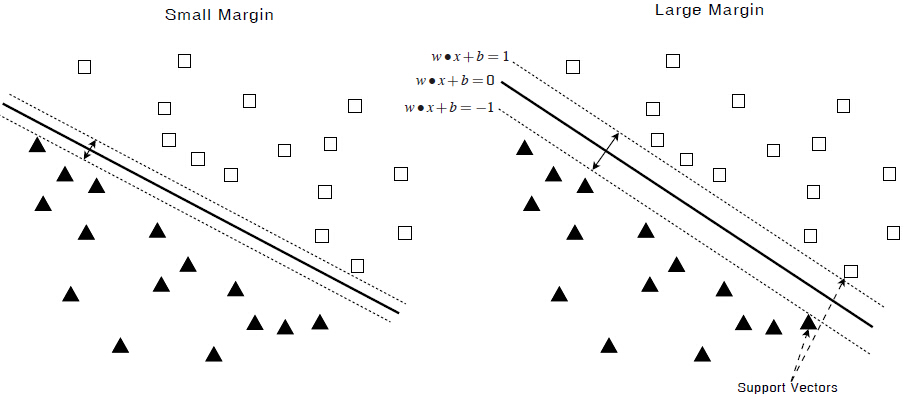
\includegraphics[scale=0.5]{f2.6.jpg}
	  	\caption{在二维上不同的边界决定可能分成不同的类。每一个边界有一个相关的边缘。}
	  \end{center}
\end{figure}

两类之间的一个线性划分是通过函数$w\cdot x+b=0$来实现的。我们定义能够划分物品类+1或是-1的函数,只要这些物品是被来自类划分函数的某个最小距离分开的。相应的函数为:
\[
f(x)=\left\{
\begin{array}{ll}
1,\ & if\ w\cdot x+b\geq 1\\
-1,\ & if\ w\cdot x+b\leq -1
\end{array}
\right.
\]

$$ Margin=\frac{2}{\|w\|^2} $$

根据SVM的主要原理,我们想要最大化两个类之间的边缘(Margin)。事实上这等价于在给定$f(x)$的条件下,最小化倒数$L(w)=\frac{\|w\|^2}{2}$。

如果物品不是线性分离的,我们可以通过引入一个松弛变量来把SVM转变为软边缘分类器。在这种情况下,新的$f(x)$和$L(w)$函数定义如下:
$$ L(w)=\frac{\|w\|^2}{2}+C\mathop{\sum}\limits_{i=1}^N\varepsilon$$

\[
f(x)=\left\{
\begin{array}{ll}
1,\ & if\ w\cdot x+b\geq 1-\varepsilon\\
-1,\ & if\ w\cdot x+b\leq -1+\varepsilon
\end{array}
\right.
\]

另一方面,如果决策边界是非线性的,我们需要转换数据到高维的空间。这个转换的完成得益于名为内核技巧的数学变换。最基本的想法是通过核函数取代在公式2.8中的点积。对于核函数有许多不同的可行的选择,比如:多项式或者是多层感知器。但是最常用的内核函数是径向基函数族(RBF)。

支持向量机最近已经在许多的环境中获得较好的性能和效率。在推荐系统里,SVM最近也显示出了显著效果。

\subsection{分类器的集成}
使用分类器集成背后的最基本的思想是,从训练数据构造一系列的分类器,并通过聚集预测值来预测类标签。只要我们能假设这些分类器都是独立的,分类器集成就有效。在这种情况下,我们可以确定分类器产生的最糟糕的结果与在集成中的最坏分类是一样的。因此,结合具有相似的分类错误的独立分类器将只会提升结果。

为了产生集成,有几种可能的方法。最常用的两个技术是Bagging和Boosting。在Bagging方法中,我们采用带替换的抽样,在每一个自举样本(bootstrap sample)上建立分类。每个样本被选择的概率为$(1-\frac{1}{N})^N$,注意如果$N$足够大,它收敛至$1-\frac{1}{e}\approx 0.623$。在Boosting 方法中,我们通过更加关注之前错误分类的记录,使用迭代过程自适应地改变训练数据的分布。一开始,所有的记录都被分配相同的权值。但是,不像Bagging 方法,在每一轮的提升中权值是可以变化的:被错误分类的记录权值将会增加,同时正确分配的记录的权值将会降低。Boosting 方法的例子是AdaBoost 算法。

分类器集成使用的例子在推荐领域里面非常的实用。事实上,任何一个混合技术都可以理解成以一种方式集成或另外几个分类器的集成。实验结果显示,集成器能产生比其它任何孤立的分类器更好的结果。

\subsection{评估分类器}
推荐系统中被接受最常用的指标是预测兴趣(评分)和测量值的均方差(MAE)或均方根误差(RMSE)。这些指标在计算精度时对推荐系统的目标没有任何假设。但是,正如McNee et al.指出的那样,除了精确度之外还有许多指标来决定物品是否要被推荐。

下一步是考虑的是,“现实”中推荐系统的目的是产生一个topN推荐列表,以及依赖于能多好地分辨出值得推荐的物品来评估这个推荐系统。如果把推荐看作分类问题,就可以使用评估分类器的著名指标,诸如:准确度和召回率。

为了评估一个模型,我们一般考虑以下的指标:真正(TP):分到类A且真的属于类A的实例数量;真负(TN):没有分到类A且真的不属于类A的实例数量;假正(FP):分到类A但不属于类A的实例数量;假负(FN):没有分到类A但属于类A的实例数量。

最常用来衡量模型性能是定义正确分类的(属于或不属于给定的类)实例和总的实例数量之间的比率:精确度=$(TP+TN)/(TP+TN+FP+FN)$但是,精确度在许多的例子中有误导。想象一个带有99900个类A的样本和100个类B的样本的两类分类问题。如果分类器简单地预测一切属于类A,计算精度可能是99.9\%,但是模型性能值得怀疑,因为它从没有发现类B中的样本。改进这种估值的一种方法是定义代价矩阵,定义将类B的样本分给类A的代价。

模型性能的其它常用指标,特别是在信息检索中,是准确率和召回率。准确率,定义为$P = TP/(TP+FP)$,是一种在分样本到类A中犯多少错误的指标。另一方面,召回率,$R = TP/(TP+FN)$,衡量没有留下本应该划分到类中的样本的程度。$F_1$指标综合了这两个指标:$F_1=\frac{2RP}{R+P}=\frac{2TP}{2TP+FN+FP}$。

有时我们会比较几个相互竞争的模型,而不是单独评估它们的性能。为此,我们使用在1950年代开发的用来分析噪音信号的技术:接受特征曲线(ROC)。ROC曲线描述了正确击中和假警告之间的特征。每一个分类的性能用曲线上的点表示(见图7)。
\begin{figure}[!htb]
	  \begin{center}
	  	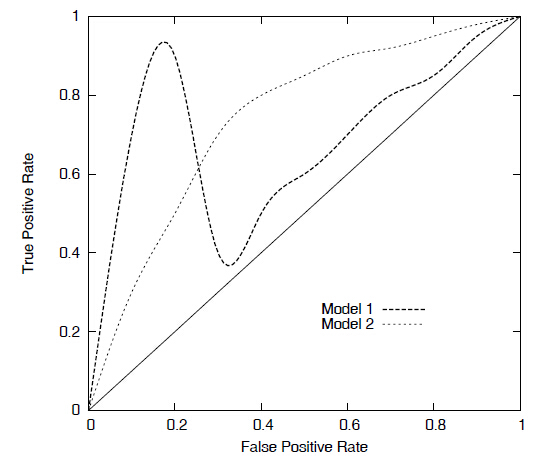
\includegraphics[scale=0.5]{f2.7.jpg}
	  	\caption{ROC曲线的例子。模型1在低假正率下表现较好,模型2的表现整体一致,在假正率高于2.5时比模型1要好。}
	  \end{center}
\end{figure}

\section{聚类分析}
聚类,也被称作为无监督的学习,分配物品到一个组中使得在同一组中的物品比不同组中的物品更加类似:目的是发现存在数据中的自然(或者说是有意义)的组。相似度是由距离衡量来决定,诸如在2.1中叙述的。聚类算法的目标是在最小化群内距离的同时最大化群间距离。

聚类算法有两个主要的类别:分层和划分。划分聚类算法把数据划分成非重合的聚类,使得每一个数据项确切在一个聚类中。分层聚类算法在已知聚类上继续聚合物品,生成聚类的嵌套集合,组成一个层级树。

许多聚类算法试图最小化一个函数来衡量聚类的质量。这样的质量函数一般被称为目标函数,因此聚类可以看作最优化的问题:理想聚类算法考虑所有可能数据划分,并且输出最小化质量函数的划分。但相应的最优化问题是NP困难问题,因此许多算法采用启发式方法(例如:k-means算法中局部最优化过程最可能结束于局部最小)。

\subsection{k-Means}
k-Means聚类是一种分块方法。函数划分$N$个物品的数据集到$k$个不相关的子集$S_j$,其中包含$N_j$个项目,以便于它们按照给定的距离指标尽可能的靠近。在分块中每一个聚类通过它的$N_j$个成员和它的中心点$\lambda_j$来定义。每一个聚类的中心点是聚类中所有其它物品到它的距离之和最小的那个点。因此,我们能把k-means定义为一个最小化$E=\sum_1^k\sum_{n\in S_j}d(x_n,\lambda_j)$的一个迭代过程,$x_n$是代表第$n$个项目的向量,$\lambda_j$是$S_j$的中心点,$d$是距离函数。

算法一开始会随机选择k个中心点。所有物品都会被分配到它们最靠近的中心节点的类中。由于聚类新添加或是移出物品,新聚类的中心节点需要更新,聚类的成员关系也需要更新。这个操作会持续下去,直到再没有物品改变它们的聚类成员关系。算法的第一次迭代的时候,大部分的聚类的最终位置就会发生,因此,跳出迭代的条件一般改变成“直到相对少的点改变聚类”来提高效率。

基础的k-means是极其简单和有效的算法。但是,它有几个缺陷:(1)为了选择合适的k值,假定有先验的数据知识(2)最终的聚类对于初始的中心点非常敏感。(3)它会产生空聚类。k-means也有几个关于数据的缺陷:当聚类是不同的大小,密度,非球状形状时,就会有问题,并且当数据包含异常值时它也会有问题。

\subsection{改进的k-Means}
基于密度的聚类算法。诸如:DBSCAN通过建立密度定义作为在一定范围内的点的数量。例如:DBSCAN定义了三种点:核心点是在给定距离内拥有超过一定数量邻居的点;边界点没有超过指定数量的邻居但属于核心点邻居;噪音点是既不是核心点也不是边界点。算法迭代移除掉噪音数据并且在剩下的点上进行聚类。

消息传递聚类算法。它是最近基于图聚类方法的系列之一。消息传递算法没有一开始就将节点的初始子集作为中心点,然后逐渐调适,而是一开始就将所有节点都看作中心点,一般称为标本。在算法执行时,这些点,现在已经是网络中的节点了,会交换消息直到聚类逐渐出现。相似传播是这种系列算法的代表,通过定义节点之间的两种信息来起作用:“责任”,反映了在考虑到其它潜在标本的情况下,接收点有多适合作为发送点的标本;“可用性”,从候选标本发送到节点,它反映了在考虑到其它选择相同标本的节点支持的情况下,这个节点选择候选标本作为其标本的合适程度。

分层聚类。它按照层级树(树枝形结构联系图)的结构产生一系列嵌套聚类。传统的分层算法使用一个相似度或者是距离矩阵来合并或者是分裂一个聚类。有两种主要方法来分层聚类。在聚集分层聚类中,我们以点作为个体聚类,并且每一个步合并最近的聚类对,直到只有一个(或是k个聚类)聚类剩下。分裂分层聚类从一个包含所有物品的聚类开始,并且每一个分裂每一聚类,直到每一聚类包含一个点(或是有K个聚类)。

就我们所知,诸如前面提到k-means的替代方法没有应用在推荐系统中。k-means算法的简单和效率优于它的替代算法。

\section{关联规则挖掘}
关联规则挖掘关注于规则的发现,其它能够根据事务中出现其它物品来预测出现某个物品。两个物品被发现相关只意味着共同出现,但是没有因果关系。

我们定义物品集为一个或多个物品的集合(例如(牛奶,啤酒,尿布))。k-物品集是包含k个物品的集合。给定物品的频繁度被称之为支持量(比如:(牛奶,啤酒,尿布)=131)。并且物品集的支持度是包含它的事务的比例(例如:(牛奶,啤酒,尿布)=0.12)。频繁物品集是支持度
大于或等于最小支持度阈值的物品集。关联规则是公式$X\Rightarrow Y$公式的表达式,其中X和Y是物品集(例如:牛奶,尿布$\Rightarrow$啤酒)。

给定一组事务集合$T$,关联规则挖掘的目标是发现具有支持度$\geq$最小支持度阈值以及置信度$\geq$最小置信度阈值的所有规则。由于暴力计算开销巨大,我们采用两步方法:(1)产生了所有支持度$\geq$ 最小支持度的物品集(频繁项集生成)。(2)从每一频繁物品集中产生高置信规则(规则产生)。

有几个技术来优化频繁物品集的产生。在一个广泛的意义上,它们可以被分成这些:尝试最小化候选集数量(M),降低事务量(N),降低比较量数量(NM)。但是最常用的方法是使用先验规
则来降低候选数量。这个原则表明如果物品集是频繁的,那么所有的子集也是频繁的。支持度的衡量标准已经验证了这一点,因为一个物品集的支持度永远不会超过它子集的支持度。Apriori算法是这个规则实际的实现。

给定一个频繁集L,产生规则时的目的是发现所有满足最小的置信度需求的非空子集。如果$|L|=k$,那么有$2k2$条候选关联规则。因此,在生成频繁物品集时,需要找到高效的方法来生成规则。对于Apriori算法,我们能通过合并规则结果中共用相同前缀的两个规则来产生候选规则。

关联规则在发现模式和推动个性化市场营销方面的显著效果闻名已久了。但是,尽管这些方法和推荐系统的目标之间有明显的关联,但是它们还是没有成为主流。主要原因是这种方法类似于基于物品的CF但缺少灵活性,因为它需要事务这个明确的概念\--事件共同出现在某个给定的会话中。

\section{总结}
本章介绍了在设计推荐系统中可能用到的主要的数据挖掘方法和技术。我们也总结了在文献中提到的用法,提供了如何以及在哪用到它们一些粗略指导。



\end{document}


